\section{Preliminaries}
\label{sectionmodel}

In this section, we first describe the network and node model.
Then we formulate the Neighbor Discovery problem formally. 
The notations are listed in Table \ref{notations}.

\begin{table}[!t]
\renewcommand{\arraystretch}{1.3}
\caption{Notations for Neighbor Discovery}
\label{notations}
\centering
\scalebox{0.92}{
\begin{tabular}{|c|c|}
\hline
\bfseries Notation & \bfseries Description\\
\hline
$u_i$ & Sensor node $u_i$ with ID $i$ \\
\hline
$t_i^s$ & Sensor node $u_i$ starts neighbor discovery at time $t_i^s$ \\
\hline
$p_n$ & A node is the neighbor of another with probability $p_n$ \\
\hline
$N$ & The number of nodes in the network is $N$ \\
\hline
$n$ & The average number of neighbors is $n$, $n=p_nN$ \\
\hline
$t_0$ & The length of a time slot is $t_0$ \\
\hline
%$\theta_i$ & Node $u_i$'s duty cycle is $\theta_i$ \\
%\hline
$L(i,j)$ & The discovery latency that node $u_i$ discovers node $u_j$ \\
\hline
$L(i)$ & The discovery latency that node $u_i$ discovers all neighbors \\
\hline
$p_i^t$ & Node $u_i$ transmits in a time slot with probability $p_i^t$ \\
\hline
$p_i^l$ & Node $u_i$ listens in a time slot with probability $p_i^l$ \\
\hline
$p_i^s$ & Node $u_i$ sleeps in a time slot with probability $p_i^s$ \\
\hline
%$p_t$ & The transmission probability as a global constant \\
%\hline
%$p_l$ & The listening probability as a global constant \\
%\hline
%$p_s$ & The sleep probability as a global constant \\
%\hline
$\theta$ & The pre-defined duty cycle is $\theta$ \\
\hline
%$p_{suc}$ & The probability that a node discovers a \\
%& neighbor successfully in a given slot is $p_{suc}$ \\
%\hline
$W$ & The time slot spent by a node discovering all neighbors is $W$ \\
\hline
%$W_j$ & The time slot spent by a node discovering a new neighbor \\
%& after it discovered j-1 neighbors is $W_j$ \\
%\hline
%$p_t(j)$ & The global transmission probability is $p_t(j)$ in $W_j$ \\
%\hline
%$p_{suc}(j)$ & The probability that a node discovers a new neighbor  \\
%& successfully in a given slot after $j-1$ neighbors is $p_{suc}(j)$ \\
%\hline
$M$ & Neighboring matrix, $M_{ij}=1$ means $u_i$ and $u_j$ are neighbors \\
\hline
\end{tabular}}
\end{table}


\subsection{Network and Node Model}

%Network connectivity
\bftext{Network connectivity.} In a large-scale network, 
since the network is deployed in a vast area, each node 
has a capacity to sense a fraction of nodes within its sensing range.
These networks are defined as \emph{Partially-Connected Networks}.

Multi-hop wireless networks are often modeled as graphs. Two nodes are connected by an 
edge if and only if the respective devices are within mutual transmission range. 
A symmetric matrix $M_{N\times N}$ is used to record the neighboring relations as:

$$ M_{i,j}=\left\{
\begin{aligned}
1  & & & & & & {connected}\\
0  & & & & & & {disconnected}\\
\end{aligned}
\right.
$$

Some communication models have been extensively studied,
such as unit-disk and SINR.

There are a few path loss model unit-disk SINR
In the multi-hop and large-scale
networks,  

We the neighbor discovery problem under the unit-disk model, 
since it is a basic model and other models can be transformed to 
it by some means.%\cite{}  



%distribution and networks
In a network, the location of the nodes are likely to obey uniform distribution[][],
Gaussian distribution[][] or other combinatorial distributions.



Among the partially-connected networks, there is a particular type called \emph{Energy-Efficient Networks}.
A typical one of energy-efficient networks is the wireless sensor network.
The wireless sensor network consists of a number of sensors distributed separately in a target area.
The deployed sensor nodes keep their most time in sleep pattern to avoid quick energy consumption 
and wake up timely to work on duty.


When a node wake up on a time slot, it can turn to either the transmitting state or listening state. 
\begin{itemize}
\item \textbf{Transmitting state}. A node turn to transmitting state will broadcast a package containing its own identify 
information to all neighbors.
\item  \textbf{Listening state}. A node turn to listening state will monitor the frequency channel to collect its neighbors' packages.
However collision will occur when two or more neighbor nodes transmit concurrently and thus no valid information will be gathered
\end{itemize}
Transiting between the states only costs little time, compared to one complete time slot.

In our model, we denote the node set in the network as $U = \{u_1,u_2,...,u_N\}$.
Time is divided into slots of equal length $t_0$, 
which is sufficient to finish  one communication process
(transmit or receive a piece of package). In each time slot, 
a node transform its pattern according to a pre-defined duty schedule.


\begin{definition}
\textbf{Duty Schedule} is a pre-defined sequence $S=\{s^t\}_{0\leq t<T}$ of period $T$ and
$$ s^t=\left\{
\begin{aligned}
S  & & & {Sleep}\\
T  & & & {Transmit}\\
L  & & & {Listen}\\
\end{aligned}
\right.
$$
\end{definition}

 Each node construct its own duty schedule according to a specific strategy and repeats it
 until finding all the neighbors. Since the waking-up duration has a significant affect on the battery's lifetime, 
 duty cycle is utilized to restrict the energy consumption.

\begin{definition}
\textbf{Duty Cycle} represents the fraction of one period T where a node turns its radio on. It can be formulated as:

$$\theta=\frac{|\{t: 0\leq t<T, s^t \in \{T,L\}\}|}{T}.
$$
  
\end{definition}

A homogeneous energy-arrangement case is that all the nodes
in the network share a common global duty cycle $\theta$,
while each nodes holding a local duty cycle $\theta_i$ is 
a heterogeneous


\subsection{Problem Definition}

We consider a partially-connected network, 
where two nodes are neighbors if they locate within the radio range of each other. 


Each node follows its duty schedule to achieve neighbor discovery. In a synchronous scenario,
nodes start their neighbor discovery process at the same time, while in a asynchronous  scenario
all nodes start at different time slots. We focus on the asynchronous case while still applicable for the
synchronous situation.

 
Notice that the neighbor discovery process is not bidirectional, which means any pair of neighbors 
need to find each other separately. The time slots within which a node $u_i$ find one of its neighbors $u_j$ can be formulated 
as $L(i,j)$. Then we define the discovery latency that node $u_i$ discovers all neighbors as:
\begin{definition}
\textbf{Discovery Latency} of node $u_i$ is the time to discover all neighbors:
$$L(i) = \max_{j:M_{i,j}=1} L(i,j).
$$
\end{definition}

Thus the neighbor discovery problem can be formulated as:
%@@@to be modified
\begin{problem}
For a node $u_i$ with its neighbor set $S = \{u_{i1},u_{i2},...u_{ij},...\}$, 
design a strategy to construct a duty schedule, which satisfies
$\forall$ neighbor nodes $u_{ij}$ :
$$
\exists t \ s.t. :  \quad
S_i(t) = L ,
S_{ij}(t) = T,
\forall k \neq j : S_{ik}(t) \in \{L, S\}.
$$

\end{problem}
%@@@

\begin{figure}[!h]
\centering
\subfigure[The topology of a wireless networks ]{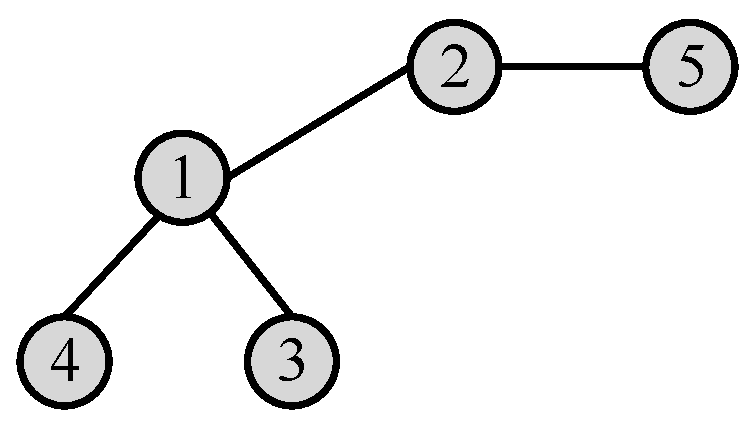
\includegraphics[width=1.65in]{./Figure/topology.eps}}
\vspace{0.03in}
\subfigure[Neighbor discovery process]{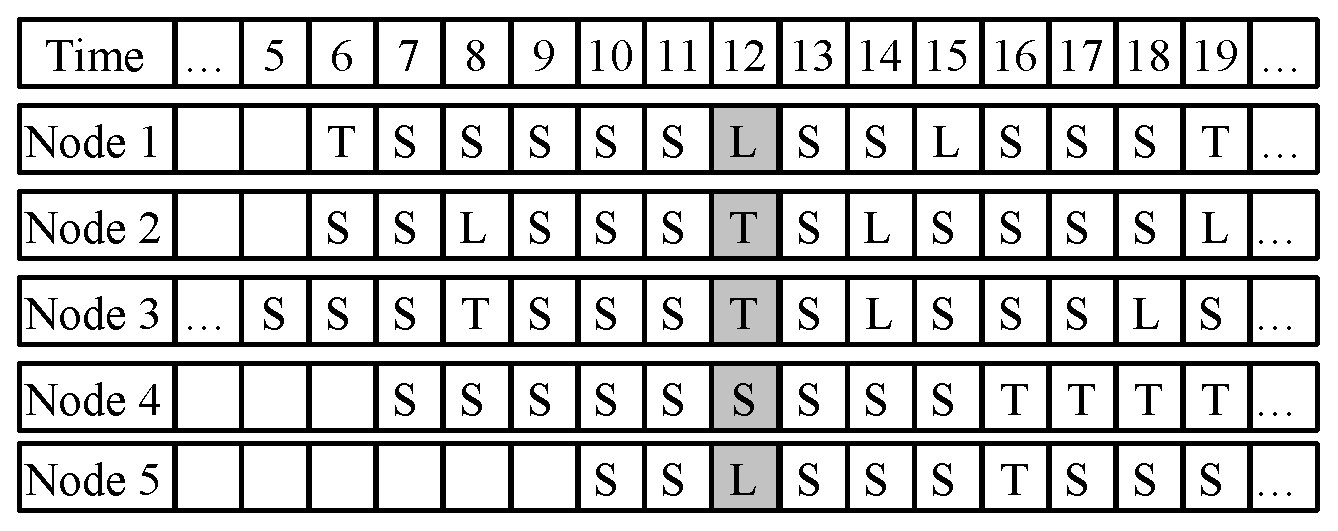
\includegraphics[width=2.8in]{./Figure/NBexample.eps}}
\caption{An example of neighbor discovering process. S, T and L represents Sleep pattern, 
Transmitting state and Listening state in wake-up pattern respectively.}
\label{NDexample}
%\vspace{-0.2in}
\end{figure}

An example of neighbor discovery process is given in Fig.\ref{NDexample}. 
Fig.\ref{NDexample}(a) shows the topology of a partially-connected 
wireless sensor network, which consists of $5$ sensor nodes. 
Fig.\ref{NDexample}(b) describes the neighbor discovery process 
in the asynchronous scenario, as we can see the nodes 
start their process at different time slot. The duty schedule of 
node $1$, for example, is $S_1 = \{ 1, 0, 0, 0, 0, 0, 1, 0, 0, 1, 0, 0, 0, 1, ... \}$.  
At time slot $12$, node 5 find its neighbor node $2$ while node $1$ 
could not find node $2$ due to a collision from its another neighbor node $3$. 



